%
% File acl2017.tex
%
%% Based on the style files for ACL-2015, with some improvements
%%  taken from the NAACL-2016 style
%% Based on the style files for ACL-2014, which were, in turn,
%% based on ACL-2013, ACL-2012, ACL-2011, ACL-2010, ACL-IJCNLP-2009,
%% EACL-2009, IJCNLP-2008...
%% Based on the style files for EACL 2006 by
%%e.agirre@ehu.es or Sergi.Balari@uab.es
%% and that of ACL 08 by Joakim Nivre and Noah Smith

\documentclass[11pt,a4paper]{article}
\usepackage[hyperref]{acl2017}
\usepackage{times}
\usepackage{latexsym}
\usepackage{graphicx}
\usepackage{url}
\usepackage{float}
\aclfinalcopy % Uncomment this line for the final submission
%\def\aclpaperid{***} %  Enter the acl Paper ID here

%\setlength\titlebox{5cm}
% You can expand the titlebox if you need extra space
% to show all the authors. Please do not make the titlebox
% smaller than 5cm (the original size); we will check this
% in the camera-ready version and ask you to change it back.

\newcommand\BibTeX{B{\sc ib}\TeX}

\title{Language Understanding System Final Project}

\author{Ardino Pierfrancesco \\
  University of Trento \\
  {\tt pierfrancesco.ardino@studenti.unitn.it}}

\date{}

\begin{document}
\maketitle
\begin{abstract}
    The extraction of concepts from a sequence of word is a fundamental task for any Spoken Language Understanding system. This document reports the work done for the final project of the LUS course at the University of Trento. The objective of this project is to compare the performance of discriminative model against the results of the generative model obtained in the Mid-Term project. Recurrent Neural Networks (RNNs) and Conditional Random Fields (CRFs) have been used as discriminative methods for this project.
\end{abstract}


\section{Introduction}

The aim of this final project is to compare the performance of generative and discriminative model for sequential labelling in the movie domain. The sequential labelling is a problem that aims at assign a domain-related tag in IOB notation to each word is a sentence. The performances of the generative model have been computed during the Mid-Term project of this course. In particular, Weighted Finite State Transducers (WFSTs) have been used as generative models. For the discriminative models, two approaches have been selected; the first one is based on Conditional Random Fields (CRF), while the second is based on Recurrent Neural Networks (RNN). The following section will talk about CRFs and the templates developed for their training. Then the third section will talk about RNNs and their performance. The last section will present the results and the comparison between the generative and the discriminative methods.

\section{Conditional Random Fields}

Discriminative models aim at computing the posterior probability $P (y|x)$
while generative models model the joint distribution $P(x,y)$ taking in account also the prior probability $P(x)$, where $x$ is a random variable over the words of a  sentence and $y$ is random variable over the labels. In this sense discriminative models can be easier to train as they do not take in account the training samples distribution, but there is an higher risk of overfitting the training data. \\
Conditional Random Fields are log-linear models\cite{elkan2008log}.
A log-linear model describes the probability of a label $y$ given the example $x$ as:
\begin{equation}
    p(y|x;w) = \frac{exp \sum_{j = 1}^{J} w_{j}F_{j}(x, y)}{Z(x, w)}
\end{equation}

$F_{j}(x,y)$ is called \textbf{feature function}. A feature function can be explained as a measure of the compatibility of the example $x$ and the label $y$. \\
The corresponding weight $w_{j}$ describes the influence of $F_{j}$.
Finally $Z(x,w)$ is a normalization factor described as:
\begin{equation}
    Z(x,w) = \sum_{y \in Y} exp \sum_{j = 1}^{J} w_{j}F_{j}(x, y)
\end{equation}
In CRF, the features function are defined as:

\begin{equation}
    F_{j}(X,Y) = \sum_{i=1}^{n} f_{j}(y_{i-1}, y_{i}, x, i)
\end{equation}
where $x$ is the sentence, $y_{i}$ is the current label, $y_{i-1}$ is the previous label and $i$ is the position. The output of a feature function is usually binary, 1 if there is a match, 0 otherwise.\\
The tool used to generate the templates to create the feature function and use them into CRFs is CRF++.
\subsection{Words}
\label{words}
The first tests was made by using the basic dataset which is composed only by words and output concepts.
The first step was to define a baseline score to be used as comparison with the other results. For this, the following template has been created:
\begin{table}[H]
    \begin{center}
        \begin{tabular}{|c|}
            \hline \bf Unigram \\ \hline
            U00:\%x[0,0] \\
            \hline
        \end{tabular}
    \end{center}
    \caption{\label{t00} Baseline template}
\end{table}
This template consider for each word of the sentence only the word itself and the label. As expected the result for this test was very low, Table \ref{t1} shows the results of the baseline
\begin{table}[H]
    \begin{center}
        \begin{tabular}{|c|c|c|c|}
            \hline \bf Accuracy &   \bf Precision &  \bf Recall &  \bf F1-Score   \\ \hline
            87.59\% & 44.99\% & 60.49\% & 51.60\%\\
            \hline
        \end{tabular}
    \end{center}
    \caption{\label{t1} Baseline score}
\end{table}

After that, the windows size has been enlarged including more and more neighbors resulting in the following template as the best for the Unigram
\begin{table}[H]
    \begin{center}
        \begin{tabular}{|c|}
            \hline \bf Unigram \\ \hline
            U00:\%x[-3,0] \\
            U01:\%x[-2,0] \\
            U02:\%x[-1,0] \\
            U03:\%x[0,0] \\
            U04:\%x[1,0] \\
            U05:\%x[2,0] \\
            \hline
        \end{tabular}
    \end{center}
    \caption{\label{t2} Best template for unigram}
\end{table}
which means that for each word \textit{w} the three preceding words and the two following words have been used to compute the concept associated to \textit{w}.
\begin{table}[h]
    \begin{center}
        \begin{tabular}{|c|c|c|c|}
            \hline \bf Accuracy &   \bf Precision &  \bf Recall &  \bf F1-Score   \\ \hline
            93.51\% & 78.81\% & 74.34\% & 76.51\%\\
            \hline
        \end{tabular}
    \end{center}
    \caption{\label{t3} Best unigram window size score}
\end{table}

Table \ref{t3} shows the results of the this template, as can be seen the F1-score has increased by over the 20\%.
After that the best window size for the bigram has been found by following the same strategy used before. The resulting template has a unigram  window size in the range $n \in [-2,3]$ and a bigram window size in the range $n \in [-2,1]$. In this case the results are the following:
\begin{table}[H]
    \begin{center}
        \begin{tabular}{|c|c|c|c|}
            \hline \bf Accuracy &   \bf Precision &  \bf Recall &  \bf F1-Score   \\ \hline
            94.03\% & 87.53\% & 77.18\% & 82.03\%\\
            \hline
        \end{tabular}
    \end{center}
    \caption{\label{t31} Best bigram window size score}
\end{table}
which as can be seen are much better than the ones obtained using only unigram rules.

In order to increase the performance some complex macros have been created by concatenating features. Concatenating the current word \textit{w} with the following word resulted in the following performance:
\begin{table}[H]
    \begin{center}
        \begin{tabular}{|c|c|c|c|}
            \hline \bf Accuracy &   \bf Precision &  \bf Recall &  \bf F1-Score   \\ \hline
            94.11\% & 88.11\% & 77.45\% & 82.44\%\\
            \hline
        \end{tabular}
    \end{center}
    \caption{\label{t4} Best only Words score}
\end{table}

as can be seen, the usage of this concatenation increased the F1-Score by +0.41\%

\subsection{Additional Features}
\subsubsection{POS}
The next step was to try the other features provided in addition to the basics set. The first features used to enrich the dataset are the POS tags of the words. Using the best template of the previous experiment and adding rules to include the POS tag in the range $n \in [-1,1]$ and a concatenation of the current word with its POS tag increased the performance by +0.50\%.
\begin{table}[H]
    \begin{center}
        \begin{tabular}{|c|c|c|c|}
            \hline \bf Accuracy &   \bf Precision &  \bf Recall &  \bf F1-Score   \\ \hline
            94.52\% & 86.70\% & 79.47\% & 82.93\%\\
            \hline
        \end{tabular}
    \end{center}
    \caption{\label{t5} Best Word-Pos score}
\end{table}
As can be seen from table \ref{t5} the result of the Precision compared to the results obtained in table \ref{t4} decrease but the F1-Score value increase thanks to an higher value for the Recall.
\subsubsection{Lemma}
The same procedure done before is repeated for the Lemma. Again, starting from the best result obtained in Section \ref{words} and adding a rule that take into consideration the lemma of the current word improved the results obtained using only the words but they are lower w.r.t. the ones obtained using POS.
\begin{table}[H]
    \begin{center}
        \begin{tabular}{|c|c|c|c|}
            \hline \bf Accuracy &   \bf Precision &  \bf Recall &  \bf F1-Score   \\ \hline
            94.25\% & 87.46\% & 78.64\% & 82.82\%\\
            \hline
        \end{tabular}
    \end{center}
    \caption{\label{t6} Best Word-Lemma score}
\end{table}

Table \ref{t6} shows the results of this experiment, as can be seen only the Precision is better w.r.t. the results obtained in Table \ref{t5}

\subsection{Pos and Lemma}
\label{PL}
In this case Lemma and POS are used jointly as additional features. As before, adding some rules about Lemma and POS and concatenation between them ends in the following template:
\begin{table}[H]
    \begin{center}
        \scalebox{0.8}{
        \begin{tabular}{|c|c|}
            \hline \bf Unigram & \bf Bigrams \\ \hline
            U00:\%x[-2,0] & B \\
            U01:\%x[-1,0] & B00:\%x[-2,0] \\
            U02:\%x[0,0] &  B01:\%x[-1,0] \\
            U03:\%x[1,0] & B02:\%x[0,0] \\
            U04:\%x[2,0] & B03:\%x[1,0] \\
            U05:\%x[3,0] &\\
            U06:\%x[0,0]/\%x[1,0] &\\
            U07:\%x[0,1] &\\
            U08:\%x[0,2] &\\
            U09:\%x[-1,1] &\\
            U10:\%x[0,0]/\%x[0,1] &\\
            U11:\%x[-1,0]/\%x[0,0]/\%x[1,0] &\\
            U12:\%x[-1,1]/\%x[0,1]/\%x[1,1] &\\
            U13:\%x[-1,2]/\%x[0,2]/\%x[1,2] &\\
            \hline
        \end{tabular}
        }
    \end{center}
    \caption{\label{t7} Best template for Word+Pos+Lemma}
\end{table}
as can be seen there are concatenation of Word, Lemma and Pos in the range $n \in [-1,1]$, this template leads to the following results:
\begin{table}[H]
    \begin{center}
        \begin{tabular}{|c|c|c|c|}
            \hline \bf Accuracy &   \bf Precision &  \bf Recall &  \bf F1-Score   \\ \hline
            94.69\% & 86.90\% & 79.65\% & 83.12\%\\
            \hline
        \end{tabular}
    \end{center}
    \caption{\label{t8} Best Word-Lemma-Pos score}
\end{table}
\subsection{Prefix and Suffix}
Another test was done by extracting prefix and suffix from the words in the basic training set. The first three letters and the last three letters of the word are taken as prefix and suffix. If prefix and suffix can not be extracted from the words a default prefix and suffix is assigned to it.
The following template is the one that gives the best results among all the test made.
\begin{table}[H]
    \begin{center}
        \scalebox{0.8}{
        \begin{tabular}{|c|c|}
            \hline \bf Unigram & \bf Bigrams \\ \hline
            U00:\%x[-2,0] & B \\
            U01:\%x[-1,0] & B00:\%x[-2,0] \\
            U02:\%x[0,0] &  B01:\%x[-1,0] \\
            U03:\%x[1,0] & B02:\%x[0,0] \\
            U04:\%x[2,0] & B03:\%x[1,0] \\
            U05:\%x[3,0] &\\
            U06:\%x[0,0]/\%x[1,0] &\\
            U07:\%x[0,1] &\\
            U08:\%x[0,2] &\\
            U09:\%x[-1,1] &\\
            U10:\%x[0,0]/\%x[0,1] &\\
            U11:\%x[-1,0]/\%x[0,0]&\\
            U12:\%x[-1,1]/\%x[0,1]&\\
            U13:\%x[-1,0]/\%x[0,0]/\%x[1,0] &\\
            U14:\%x[0,3] &\\
            U15:\%x[0,4] &\\
            \hline
        \end{tabular}
        }
    \end{center}
    \caption{\label{t9} Best template for Prefix+ Suffix}
\end{table}
As can be seen other than using basics rule for the additional features, there are concatenation of the current word with its POS, of the current word with its following words, a concatenation of the previous POS with the current POS, a concatenation of the previous word and the current word and a combination of the current word with its preceding word and its following word. This template leads to the following result:
\begin{table}[H]
    \begin{center}
        \begin{tabular}{|c|c|c|c|}
            \hline \bf Accuracy &   \bf Precision &  \bf Recall &  \bf F1-Score   \\ \hline
            94.70\% & 86.96\% & 80.66\% & 83.69\%\\
            \hline
        \end{tabular}
    \end{center}
    \caption{\label{t10} Best Word-Lemma-Pos score}
\end{table}

\subsection{Other Test}
Other tests were made by changing the \texttt{eta} parameter of the CRF model, but unfortunately the best results were given by the model with the default parameter. Using the enhanced dataset, without the O concept, used during the training of the generative model in the Mid-Term-Project was not feasible as CRF++ crashed as soon as the program started due to the high number of features in the model.
\section{Recurrent Neural Networks}
\label{sec:RNN}
In traditional Neural Networks (NN) inputs and outputs are independent of each other. This is good for some tasks, but for others,i.e. exploit sequential information, can be a bad idea. For examples in sequence labelling is better to know which words come before in order to predict the next tag. In order to overcome this problem Recurrent Neural Networks (RNNs) are used. They are a class of Neural Network where connections between units form a directed cycle. This creates an internal state of the network which allows it to exhibit dynamic temporal behavior.\\
RNNs are called recurrent because they perform the same task for every element of a sequence, with the output being depended on the previous computations.

\begin{figure}[h]
    \centering
    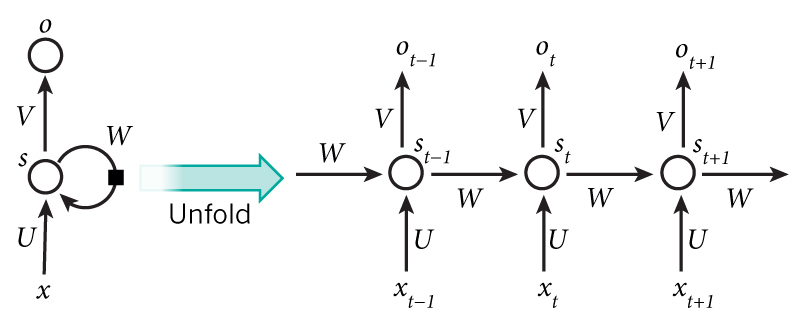
\includegraphics[width=0.5\textwidth]{rnn.png}
    \caption{A recurrent neural network and its unfolding}
    \label{RNNExample}
\end{figure}

Figure \ref{RNNExample} shows an example of the unrolling of a RNN. Unrolling means write the network for the complete sequence. For example, if the sequence is a sentence of 5 words, the network would be unrolled into a 5-layer neural network, one layer for each word. The formulas that govern the computation happening in a RNN are as follows:

\begin{itemize}
    \item $x_{t}$ is the input at step \textit{t}
    \item $s_{t}$ is the hidden state, i.e. the memory of the network, at step \textit{t}
    \item $o_{t}$ is the output at step \textit{t}
\end{itemize}
During the course two type of RNNs have been seen, Elman RNN and Jordan RNN. The two RNNs differs on the kind of recursion. The Elman RNN models the posterior probability of the concept at time \textit{t} taking as input the word at position \textit{t} and the output of the previous Hidden Layer at time \textit{t-1}. On the other hand the Jordan RNN models the posterior probability taking as input the word at position \textit{t} and the output of the previous layer, i.e. the resulting label of the previous word.\\
\subsection{RNN Hyper-parameters}
The code of the two RNNS has been provided by Dr. Ali Orkan Bayer.
The hyper-parameters of the two RNNs are the following:
\begin{itemize}
    \item \textbf{lr}: the learning rate value
    \item \textbf{win}: the context windows which is used to determine the context of each word
    \item \textbf{bs}: the number of words to be used for the backpropagation step;
    \item \textbf{nhidden}:  the number of hidden units
    \item \textbf{seed}: random seed to shuffle the examples
    \item \textbf{emb\_dimension}: the dimension of the word embedding
    \item \textbf{nepochs}: the maximum number of backpropagation steps
\end{itemize}

\subsection{Validation Set}
To avoid overfitting the training data, a validation set is used during the training phase. The validation set was not provided in the dataset, so it has been created by extracting a percentage of sentences in the training set and using them as validation set. All the experiments have been done by using as validation set 300 sentences randomly taken from the training set.
% include your own bib file like this:

\subsection{Basic Features}
At the beginning the tests have been developed using the basic dataset. Both Elman and Jordan RNN have been tested changing the hyper-parameters of the model. The result showed in table \ref{t11} are the best obtained for these tests using the default values as hyper-parameters. In fact, changing them leads to a performance drops and in some case in longer training phase, probably caused by the higher number of hidden layers.
\begin{table}[H]
    \begin{center}
        \begin{tabular}{|c|c|c|c|c|}
            \hline \bf Model &\bf Accuracy &   \bf Precision &  \bf Recall &  \bf F1-Score   \\ \hline
            Elman & 95.80\% & 80.78\% & 79.74\% & 80.26\%\\
            Jordan & 95.62\% & 81.47\% & 79.01\% & 80.22\%\\
            \hline
        \end{tabular}
    \end{center}
    \caption{\label{t11} Rnn Best score on basic set}
\end{table}
As can be seen, the Elman RNN in general performs better but the Jordan RNN is better in the Precision metric.
%\bibliographystyle{acl}
%\bibliography{acl2017}
\bibliography{acl2017}
\bibliographystyle{acl_natbib}
\subsection{Advanced Features}
After the tests with the basic dataset, the additional features provided have been used for the training. In this case, the additional features have been concatenated with the basic training set, as it has been done in the Mid-Term-Project,  in different ways:
\begin{itemize}
    \item \textbf{Word + Pos}: each word in the training set is concatenated with its POS tag
    \item \textbf{Lemma + Pos}: each lemma in the training set is concatenated with its POS tag
    \item \textbf{Word + Lemma + Pos}: Word, Lemma and POS are concatenated all together
\end{itemize}

Table \ref{t12} shows the results of the Elman and the Jordan RNNs using the concatenation of Word and Pos as features, again the default values of the hyper-parameters are used.
\begin{table}[H]
    \begin{center}
    \scalebox{0.85}{
        \begin{tabular}{|c|c|c|c|c|}
            \hline \bf Model &\bf Accuracy &   \bf Precision &  \bf Recall &  \bf F1-Score   \\ \hline
            Elman & 94.87\% & 76.99\% & 76.99\% & 76.99\%\\
            Jordan & 95.11\% & 79.68\% & 77.27\% & 78.46\%\\
            \hline
        \end{tabular}}
    \end{center}
    \caption{\label{t12} Rnn Best score on Word + Pos set}
\end{table}
As can be seen, as it was using SFST in the Mid-Term-Project, using the concatenation of Word and Pos as feature leads to a drop in performance by a $\sim$4\% for the Elman and a $\sim$\%2 for the Jordan that now outscore the Elman RNN in all the metrics.\\
Table \ref{t13} shows the results of the Elman and the Jordan RNNs using the concatenation of Lemma and Pos as features, again the default values of the hyper-parameters are used.
\begin{table}[H]
    \begin{center}
    \scalebox{0.85}{
        \begin{tabular}{|c|c|c|c|c|}
            \hline \bf Model &\bf Accuracy &   \bf Precision &  \bf Recall &  \bf F1-Score   \\ \hline
            Elman & 95.11\% & 81.57\% & 76.26\% & 78.83\%\\
            Jordan & 94.81\% & 82.61\% & 73.42\% & 77.84\%\\
            \hline
        \end{tabular}}
    \end{center}
    \caption{\label{t13} Rnn Best score on Lemma + Pos set}
\end{table}
Again, there is a drop in performance compared to the Basic set, but now the Elman RNN outscore the Jordan RNN increasing also the performance compared to Table \ref{t12}. The Jordan RNN not only has lower performance compare to the Elman RNN, but has lower performance also w.r.t the previous computation using Word and Pos.\\
Finally, Table \ref{t14} shows the results of the Elman and the Jordan RNNs using the concatenation of Word, Lemma and Pos as features, using the default values of the hyper-parameters.
\begin{table}[H]
    \begin{center}
    \scalebox{0.85}{
        \begin{tabular}{|c|c|c|c|c|}
            \hline \bf Model &\bf Accuracy &   \bf Precision &  \bf Recall &  \bf F1-Score   \\ \hline
            Elman & 94.51\% & 78.00\% & 72.14\% & 74.95\%\\
            Jordan & 94.43\% & 79.53\% & 73.69\% & 76.50\%\\
            \hline
        \end{tabular}}
    \end{center}
    \caption{\label{t14} Rnn Best score on Word + Lemma + Pos set}
\end{table}
As for the others, this test perform worse then the first. As \ref{t12} the Jordan RNN perform better than the Elman RNN. This test has the worst performance among all the tests made with RNNs, showing that probably the training set is too small for this concatenation of features.
\section{Conclusion}
During the two projects two kind of model in the context of Spoken Language Understanding have been developed and compared. The generative model (SFSTs) and
two discriminative models (CRFs and RNNs).
The comparison has been done on four metrics, Accuracy, Precision, Recall and F1-Score, with a particular attention on the latter.
The best results regarding the F1-Score (83.69\%) have been reached by the last test made with CRFs using Word, Lemma, Pos and the suffix and the prefix of the word. This result is only $\sim$1\% better than the score reached using the SFSTs (82.74\%) using the enhanced dataset with the word itself instead of the O concept while it is $\sim$3\% better than the result reached using the Elman RNN with the basic dataset.\\
The best Accuracy has been reached by the Elman RNN using the basic dataset with an Accuracy of 95.80\%, which is $\sim$1\% better than both SFST and CRF.\\
Regarding the training time, SFST is the fastest model to train. In fact, it took only $\sim$3/4 minutes for the training phase, $\sim$2 minutes faster than CRF and nearly 8 times faster than RNNs.\\
The performance of the RNN is highly influenced by the dimension of the dataset, $\sim$3300 sentences seems to be low for the training of a RNN considered  that a part of the training set has to be used for the validation set. With a larger dataset the RNNs will probably reach the same performance of the CRF.
In general it seems that CRF is the best model providing a good compromise between performance and training time.
\bibliography{references}
\bibliographystyle{acl_natbib}

\end{document}
